\documentclass{article}

% if you need to pass options to natbib, use, e.g.:
%     \PassOptionsToPackage{numbers, compress}{natbib}
% before loading neurips_2019

% ready for submission
% \usepackage{neurips_2019}

% to compile a preprint version, e.g., for submission to arXiv, add add the
% [preprint] option:
     \usepackage[preprint]{neurips_2019}

% to compile a camera-ready version, add the [final] option, e.g.:
%     \usepackage[final]{neurips_2019}

% to avoid loading the natbib package, add option nonatbib:
%     \usepackage[nonatbib]{neurips_2019}

\usepackage[utf8]{inputenc} % allow utf-8 input
\usepackage[T1]{fontenc}    % use 8-bit T1 fonts
\usepackage{hyperref}       % hyperlinks
\usepackage{url}            % simple URL typesetting
\usepackage{booktabs}       % professional-quality tables
\usepackage{amsfonts}       % blackboard math symbols
\usepackage{nicefrac}       % compact symbols for 1/2, etc.
\usepackage{microtype}      % microtypography
\usepackage{graphicx}
\usepackage{algorithm}
\usepackage{algorithmic}
\usepackage{amssymb}
\renewcommand{\algorithmicrequire}{ \textbf{Input:}} %Use Input in the format of Algorithm
\renewcommand{\algorithmicensure}{ \textbf{Output:}} %UseOutput in the format 


\title{Friends recommendation based on link prediction in social network}

% The \author macro works with any number of authors. There are two commands
% used to separate the names and addresses of multiple authors: \And and \AND.
%
% Using \And between authors leaves it to LaTeX to determine where to break the
% lines. Using \AND forces a line break at that point. So, if LaTeX puts 3 of 4
% authors names on the first line, and the last on the second line, try using
% \AND instead of \And before the third author name.

\author{%
  	CHONG Ka Hung\\
  	20543539\\
	\texttt{khchongac@connect.ust.hk} \\
	\And
	HUANG Qiuyu\\
	20548333\\
	\texttt{qhuangak@connect.ust.hk}\\
	\AND
	WANG Yutong\\
	20541402\\
	\texttt{ywangix@connect.ust.hk}\\
	\And
	YANG Yue\\
	20549600\\
	\texttt{yyangdh@connect.ust.hk}\\
  % examples of more authors
  % \And
  % Coauthor \\
  % Affiliation \\
  % Address \\
  % \texttt{email} \\
  % \AND
  % Coauthor \\
  % Affiliation \\
  % Address \\
  % \texttt{email} \\
  % \And
  % Coauthor \\
  % Affiliation \\
  % Address \\
  % \texttt{email} \\
  % \And
  % Coauthor \\
  % Affiliation \\
  % Address \\
  % \texttt{email} \\
}

\begin{document}

\maketitle

\begin{abstract}
Online social networks like Facebook recommend new friends to registered users based on local features of the graph. Link prediction in social networks has attracted increasing attention in the physical and computer science community and is a key problem for network-structured data and use some score functions, such as common neighbors and Katz index to measure the likelihood of links. The algorithms can be used to extract missing information, recommend friends in social networks, and so on. This project aims to use link prediction to recommend friends to people in the complex social networks, and there are 6 different algorithms related to the link prediction implemented and discussed. Finally, we summarize the performance of different link prediction algorithms and compare the prediction results. 
\end{abstract}

\section{Introduction}
Link prediction in the network aims to predict both present unknown links and the likely future links. Link prediction problems are widely concerned by scientists from different fields and with different backgrounds, first and foremost because of their significant practical application value. The research ideas and methods are mainly based on Markov chain and machine learning.There are many methods applied in link prediction. Literature [1] applies Markov chain for network link prediction and path analysis. Later, the literature [2] extended the Markov chain-based prediction method to the prediction of adaptive web sites. In addition,some models focus on more information to explore the network.For example,the literature [3] proposes a regression model to predict the citation relationship of scientific literature in the literature citation network which not only uses the information of the citation network, but also the external information such as author information, journal information and article content. Prediction of application node attributes. By using the topology information of the network and the attributes of the nodes, a local conditional probability model is established for prediction[4]. Besides, the similarity between nodes based on the attributes of nodes, which can be directly used for link prediction[5]. \\

Although the external information such as node attributes can be helpful to be well predicted in many cases, the acquisition of information is very difficult and sometimes even impossible where the user information in many online systems is confidential. In addition, even if the attribute information of the node is obtained, it is difficult to ensure the reliability of it, whether the attribute reflects the real situation of the node. For example, even in the social network, the registration information of many users is fake. In the case where accurate information of the node attributes can be obtained, and how to identify which information is useful for network link prediction and which information is useless is still a problem. In recent years, network structure-based link prediction methods have became more popular. The structure of the network is easier to obtain and more reliable than the attribute information of the node. In 2008, the literature [6] proposed a method for link prediction using the hierarchical structure of the network, and performed well in a network with a distinct hierarchical structure. \\

Link prediction not only has a wide range of practical applications, but also has important theoretical research significance. In recent years, with the rapid development of network science, the research of link prediction is closely related to the structure and evolution of the network. Therefore, the predicted results can be explained from a theoretical perspective. At the same time, the research of link prediction can theoretically help people understand the mechanism of complex network evolution.This project uses a machine learning method GBDT (Gradient Boosting Decision Tree) and five typical similarity prediction algorithms, namely common neighbor, Jaccard coefficient,  Adamic-Adar index, preferential attachment, and the Katz index to do the link prediction and comparative analysis.
	

\section{Objective}
In the Link prediction problem of social networks, we usually consider the special features of social networks. Social networks have a couple of interesting properties, such as:\\
\paragraph{Power law degree distribution:}most people have very few links, but a small number of people have far more links than others.\\
%\begin{figure}[h!]
%	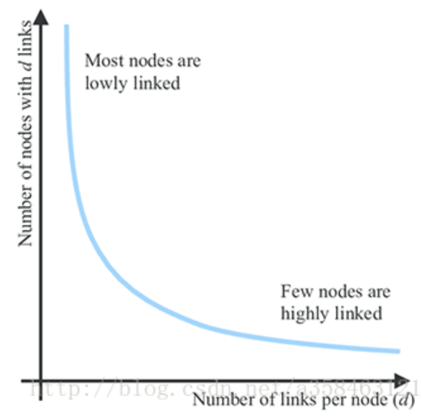
\includegraphics[width=5cm]{images/power_law.png}
%	\centering
%	\caption{Power Law.}\label{power}
%\end{figure}

\paragraph{Small-world Phenomenon:}also known as a six-degree space, there are no more than six people between you and a stranger.\\

\paragraph{Community structure (clustering effect):} within a social network, there are many small groups that all know each other.\\

So how to do the link prediction, the traditional methods are path-based Methods, neighbor-based Methods, etc. In this project, we have tried to learn the principle of this two parts of link prediction algorithm, including common neighbors, Jaccard’s coefficient, Adamic/ Adar and preferential attachment algorithm in neighbor-based methods, and Katz algorithm in path-based methods.\\ 


We have realized those algorithm by ourselves, and we have tried to realize a GBDT model which is using the index generated by above different traditional methods as features to predict the existence of an edge.
\\

After realized those algorithm, we have compared the accuracy of each link prediction algorithm and used them to do some prediction for nodes.
\\

\section{Dataset}
In this project, we crawled the Facebook website, for each user $u$, we traverse all his friends and then traverse the friends of each of $u$’s friends etc.\\

We created a data set with 4039 users, and 88234 edges and stored in a .txt file which is 854KB. The density of the whole social graph made by this nodes is 0.01082. 
\\

At the same time, we counted the degrees of each node and classified them according to the degrees of the nodes. We found that there were 75 users with only one friend, 790 users with between one and 10, 2683 users with more than 10 friends but less than 100, and 491 users with more than 100 friends. The users with the most friends had 1,045. As the bar graph shows below:
\\
\begin{figure}[h!]
	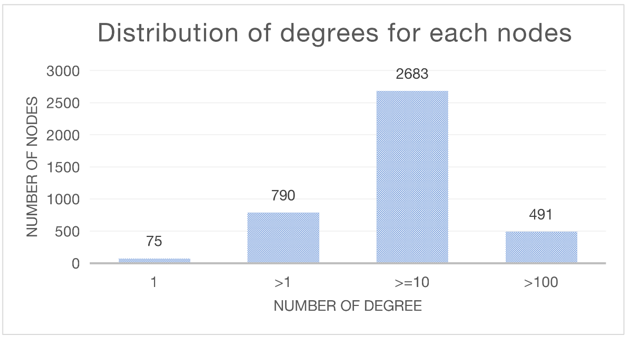
\includegraphics[width=10cm]{images/distribution.png}
	\centering
	\caption{The distribution of  degrees for each nodes.}\label{dis}
\end{figure}

To test our code, we catch part of the node and edge randomly in the total data set, which include 1820 nodes and 7084 edges and the density of the graph is 0.00428.\\ 


In this social network, it contains 1,099 nodes with one friend, 363 nodes with no more than 10 friends, 350 nodes with no more than 100 friends, and eight nodes with more than 100 friends. As the follow graph shows:
\\

\begin{figure}[h!]
	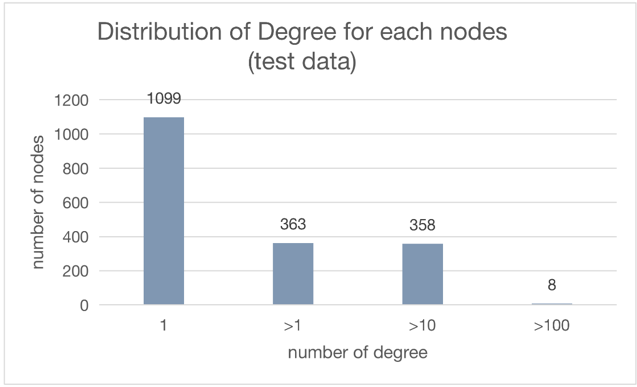
\includegraphics[width=10cm]{images/test_distri.png}
	\centering
	\caption{The Distribution of Degree for each nodes in test data.}\label{test}
\end{figure}

In the code, we divided the data file into training data and test data according to the ratio of 8:2.\\

\section{Methodology}
Social networks are very complex, and most networks are constantly changing dynamically in real time. For example, there are always new people to join the group, new contacts to be created, and old contacts or nodes to be deleted. Link prediction is very important for data mining and analysis of social networks.\\

The existing link prediction approaches can be classified into similarity-based ones and learning-based ones, and similarity-based approaches are to compute the similarities between a pair of nodes by various graph-based similarity metrics and to use the ranking on the similarity scores to predict the link between two vertices[7]. The learning-based approach is to consider link prediction as a classification task, using a classical machine learning model to learn this classification task. This project uses a machine learning method GBDT (Gradient Boosting Decision Tree) and five typical similarity prediction algorithms, namely common neighbors, Jaccard index,  Adamic/Adar index, preferential attachment, and the Katz index.\\

\subsection{Common Neighbors}
The link prediction algorithm with node similarity has low time complexity and high prediction accuracy, and is one of the most widely used link prediction algorithms. The common neighbor algorithm is widely used in the node similarity algorithm. The concept of this algorithm is very simple. When two users have many common neighbors, we tend to think that the two users are likely to establish a connection. As shown in Figure \ref{CN_NW}, point U and point V have three common neighbors which occupy most of their neighbors, so we think point U and point V are likely to be friends.

\begin{figure}[h!]
	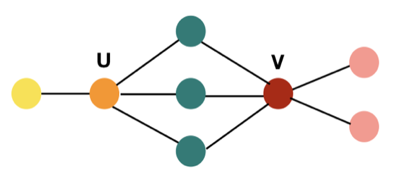
\includegraphics{images/nearest.png}
	\centering
	\caption{Shared Nearest Neighbors.}	\label{CN_NW}
\end{figure}

Hence the similarity of the two users can be expressed by the number of their neighbors:\\
\begin{equation}
Score(x,y) = |\Gamma (x) \cap \Gamma (y)|
\end{equation}


Where $\Gamma(x)$ is the node set x adjacent to the node, and $\Gamma(y)$ is the node set y adjacent to the node. A value of 0 means that the two nodes are not close, and a higher value means that the nodes are closer.  The algorithm is listed in Algorithm \ref{CN}.\\

\begin{algorithm}[htb] 
	\caption{Common Neighbor} 
	\label{CN} 
	\begin{algorithmic}
		\REQUIRE  	graph $G(V,E);$
		\ENSURE  matrix of similarity $S \in \mathbb{R}^{n \times n};$
		\STATE Initialization: $S;$ 
		\FOR{$i=1 \to n$}
		\FOR{$j=1 \to n$}
		\STATE$\mathcal{S}_t(v_i,v_j) \gets  | \Gamma(v_i) |  \cap  | \Gamma(v_j) |;$
		\ENDFOR
		\ENDFOR
		\RETURN $S;$
	\end{algorithmic}
\end{algorithm}

\subsection{Jaccard Coefficient}
Although common neighbors can help us find likely friends, however, it can be unreliable sometimes. Consider a situation,if one person has a lot of neighbors, then everyone will tend to predict interaction with him. In order to solve this problem, the number of neighbors has to be taken into account. Jaccard used a coefficient to describe how to find the similarity[8]. That is if the greater the number of same neighbors in two people, the greater the proportion of all their friends, the more likely they are to be connected. As shown in the Figure \ref{JC_NW}, Z has many neighbors so it tends to be connected with other nodes, however according to the Jaccard theorem, Y and X have stronger connection. \\

\begin{figure}[h!]
	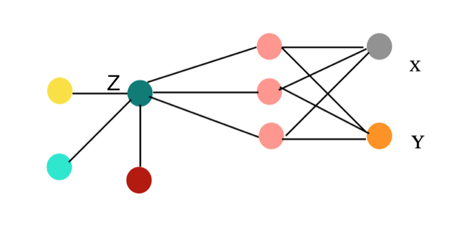
\includegraphics[width=7cm]{images/jc_nw.png}
	\centering
	\caption{Sample Network of Jaccard Coefficient.}	\label{JC_NW}
\end{figure}

The Jaccard coefficient is the number of the same neighbors of y and x divide the number of their all neighbors, which can help to find the accuracy similarity of the nodes.The algorithm is listed in Algorithm \ref{JC}. \\

\begin{algorithm}[htb] 
	\caption{Jaccard Coefficient} 
	\label{JC} 
	\begin{algorithmic}
		\REQUIRE  	graph $G(V,E);$
		\ENSURE  matrix of similarity $S \in \mathbb{R}^{n \times n};$
		\STATE Initialization: $S;$ 
		\FOR{$i=1 \to n$}
		\FOR{$j=1 \to n$}
		\STATE$\mathcal{S}_t(v_i,v_j) \gets  \frac{| \Gamma(v_i) |  \cap  | \Gamma(v_j) |}{ | \Gamma(v_i) |  \cup  | \Gamma(v_j) |};$
		\ENDFOR
		\ENDFOR
		\RETURN $S;$
	\end{algorithmic}
\end{algorithm}

\subsection{Adamic Adar}
Another method which is also an improvement on common neighbors. When we calculate the number of two identical neighbors, the importance of each neighbor is different. Assume that the fewer the neighbors of this node, the more important it is to be a center. For example, although x and y have some common neighbors, x has weaker evidence for each neighbor, and by contrast y has fewer neighbors which means it gives more importance for each neighbor. \\

\begin{figure}[h!]
	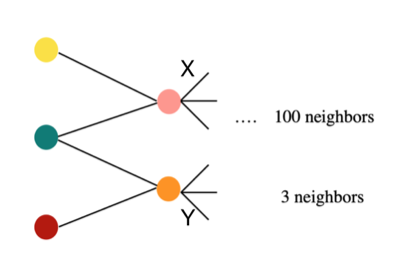
\includegraphics[width=6cm]{images/aa_nw.png}
	\centering
	\caption{Example of Adamic Adar method.}	\label{AA_NW}
\end{figure}

 Therefore, the idea of the Adamic Adar algorithm is that the contribution of common neighbor node with a small degree is greater than the common neighbor node with a large degree. For example, in a social network, the probability of connecting two people who are concerned about a relatively unpopular topic tends to be higher than the probability of connecting people who are concerned about the same hot topic. In this case, each node is given a weight value according to the degree of the common neighbor node.The algorithm is listed in Algorithm \ref{AA}.
 
 
 \begin{algorithm}[htb] 
 	\caption{Adamic Adar} 
 	\label{AA} 
 	\begin{algorithmic}
 		\REQUIRE  	graph $G(V,E);$
 		\ENSURE  matrix of similarity $S \in \mathbb{R}^{n \times n};$
 		\STATE Initialization: $S;$ 
 		\FOR{$i=1 \to n$}
 		\FOR{$j=1 \to n$}
 		\STATE$\mathcal{S}_t(v_i,v_j) \gets  \sum\limits_{z \in \Gamma(v_i)  \cap  \Gamma(v_j) }\frac{1}{ log| \Gamma(z)|};$
 		\ENDFOR
 		\ENDFOR
 		\RETURN $S;$
 	\end{algorithmic}
 \end{algorithm}

\subsection{Preferential Attachment}
In social networks, it is obvious that new nodes prefer to attach to well-connected nodes over less-well connected nodes. The simple point is that users with more friends will be more inclined to create more connections. For example, as shown in Figure \ref{PA_NW}, B is more likely to establish a connection with C than to establish a link with A. It can be noted that this similarity calculation does not require neighbor information for any node, so the algorithm has the lowest computational complexity in the similarity algorithm. \\

\begin{figure}[h!]
	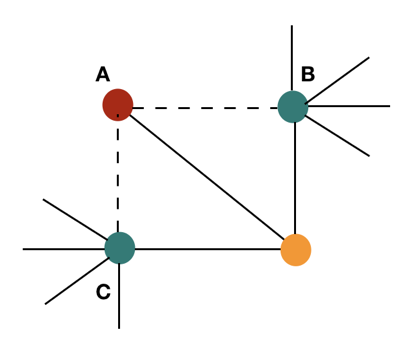
\includegraphics[width=5cm]{images/pa_nw.png}
	\centering
	\caption{Sample Network of Preferential Attachment.}	\label{PA_NW}
\end{figure}

The similarity of the two users can be expressed by the product of the number of friends:
\begin{equation}
Score(x,y) = |\Gamma (x)|*| \Gamma (y)|
\end{equation}

It estimate how  ”rich”  two vertices are by calculating the multiplication between the number of friends or followers each vertex has. Where $|\Gamma(x)|$ is the number of friends of x, and $|\Gamma(y)|$ is the number of friends of y. A value of 0 means that the possibility of establishing a connection between two points is very low, and a higher value means that the possibility is higher. The algorithm is listed in Algorithm \ref{PA}.

\begin{algorithm}

	\caption{ Preferential Attachment}

	\label{PA} 
	\begin{algorithmic}

		\REQUIRE
		graph $G(V,E)$,

		\ENSURE

		matrix of similarity $S \in \mathbb{R}^{n \times n}$

		\STATE Initialization: $S;$

		\FOR{$i=1$ $\to$ $n$}

		\FOR{$j=1$ $\to$ $n$}

		\STATE $\mathcal{S}_t(v_i,v_j)$ $\gets$ $|\Gamma(v_i)|$ $|\Gamma(v_j)|;$

		\ENDFOR	

		\ENDFOR	

		\STATE \RETURN $S;$

	\end{algorithmic}

\end{algorithm}


\subsection{Katz Centrality}

The eigenvector method performs very well on undirected graphs, but in the eigenvector centrality metric, there is such a problem: A point is heavily concerned, but the node of focus on that node is low (or even 0), which results in a node in the network that is heavily focused but has a zero centrality. In following example, when a directed acyclic graph appears, the node eigenvector centrality becomes 0. \\

\begin{figure}[h!]
	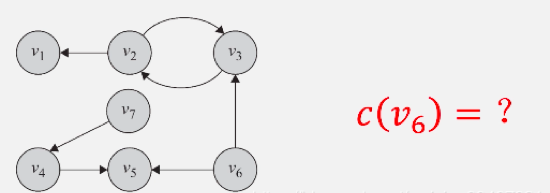
\includegraphics{images/kz_nw.png}
	\centering
	\caption{Sample Network of Katz Centrality .}	\label{KZ_NW}
\end{figure}

Katz Centrality solves this problem. Its principle is similar to eigenvector centrality, except that we provide each node with an initial value of $\beta$, which is a simple change to the formula of eigenvector centrality $x_i=k_1^{-1} \sum\limits_{i}A_{ij}x_j$ , and change to $x_i=a\sum\limits_jA_{ij}x_j+\beta$ , Where $\alpha$ and $\beta$ are constants. \\

After the matrix expression conversion, we get:

\begin{equation}
x = \alpha A x + \beta * 1
\end{equation}

\begin{equation}
x = \beta (I - \alpha A)^{-1} * 1
\end{equation}

We only care about the relative value of the centrality value, that is, regardless of whether your centrality value is 10 or 100, we only pay attention to whether your centrality value is greater than my centrality value, because we want to find the top 10 nodes with the highest centrality value. The purpose is to do rankings. Then $\beta$ can be set to 1, so Katz Centrality is expressed as: \\
\begin{equation}
x = (I - \alpha A)^{-1} * 1
\end{equation}
In fact, the ratio of $\alpha$ and $\beta$ reflects the weight of the neighbor node's centrality value. If $\alpha = 0$ then the centrality value of all nodes is $\beta = 1$, which is completely unaffected by neighbors. So this formula is more universal. \\
It should be noted that $\alpha$ can't be too big, and when $a^{-1} = k_1$  , it will result $(I - \alpha A) = 0$  , so that $(I - \alpha A)^{-1}$ can't converge. So have $0< \alpha < k_1^{-1}$. \\
To calculate Katz centrality, the inverse matrix operation is performed, and the direct computation complexity is O(n3). We can use iterative method, the formula as follow shows:\\
\begin{equation}
x(t) = \alpha A x (t - 1) + \beta * 1
\end{equation}
So that the centrality calculation method of node 5 and 6 in the above example will change to : \\

\begin{equation}
c(v_6) = \beta
\end{equation}

\begin{equation}
c(v_5) = \alpha * [c(v_4)+c(v_6)] + \beta
\end{equation}


\subsection{Gradient Boosting Decision Tree}
The last method in our project for link prediction is Gradient Boosting Decision Tree, one of the machine learning algorithm.
\subsubsection{Introduction}
Gradient Boosting Decision Tree (GBDT) is one of the  machine learning techniques for solving regression and classification problems, which is an ensemble of several weak decision trees. Like other boosting models, GBDT is in a stage-wise fashion and is able to use an arbitrary differentiable loss function to optimize those stages. \\

The problem to be tackled in this project is to recommend friends by predicting the existence of an edge between two disconnected nodes, which is actually a problem of binary classification. A two-node pair will be labeled 1 if there is an edge, and 0 otherwise. \\

Apart from the label, the next important issue is to generate features for the model. Apparently the ids of both nodes will be involved in the feature list, but that is insufficient. More features should be generated for a higher performance. Therefore we applied all the methods examined before including Common Neighbors, Preferential Attachment, Jaccard, Adamic Adar and Katz Index, as well as some other methods like Resource Allocation, Adjusted Rand, Neighborhood Distance, Total Neighbors, Same Community and U \& V Degree to calculate the index between two nodes. Then put those result indexes from different methods to the feature list for training the model. \\

\subsubsection{Data preprocessing}
Firstly we sampled the original edge list data at percentage of 70 to form the training set, and sampled 90\% again as the testing set. Besides, found out and append the missing links at distance 2 in both training and testing file. Then calculated the scores using all the methods mentioned above based on the original graph without missing links and stored the result as features for all node pairs. Finally assigned labels to them accordingly, 1 for having edge and 0 otherwise. Sample records as following:

\begin{table}[h!]
	\centering
	\caption{Sample Record}
	\begin{tabular}{cccccccccccccc}
		\hline
		nodes& label& CN& JC& AA& RA& PA& AR& ND& TN& SC& UD& VD& KZ\\
		\hline
		(0, 25)& 1& 17& 0.23& 6.11& 1.11& 1798& 0.17& 0.4& 74& 1& 62& 29& 0.00\\
		(0, 53)& 0& 1& 0.02& 0.29& 0.03& 310& -0.0014& 0.06& 66& 1& 62& 5& 0.00\\
		\hline
	\end{tabular}
\end{table}


\subsubsection{Model}
The parameters for the model are set as following:\\
\begin{table}[h]
	\centering
	\caption{Model Parameter}
	\begin{tabular}{ccccc}
		\hline
		No.estimators& Max Depth& Loss Function& Learning Rate& Subsample\\
		\hline
		300& 4& deviance& 0.03& 0.8\\
		\hline
	\end{tabular}
\end{table}

\subsubsection{Result}
After training the model, a statistics was made to examine the importance of each feature. \\
\begin{figure}[h!]
	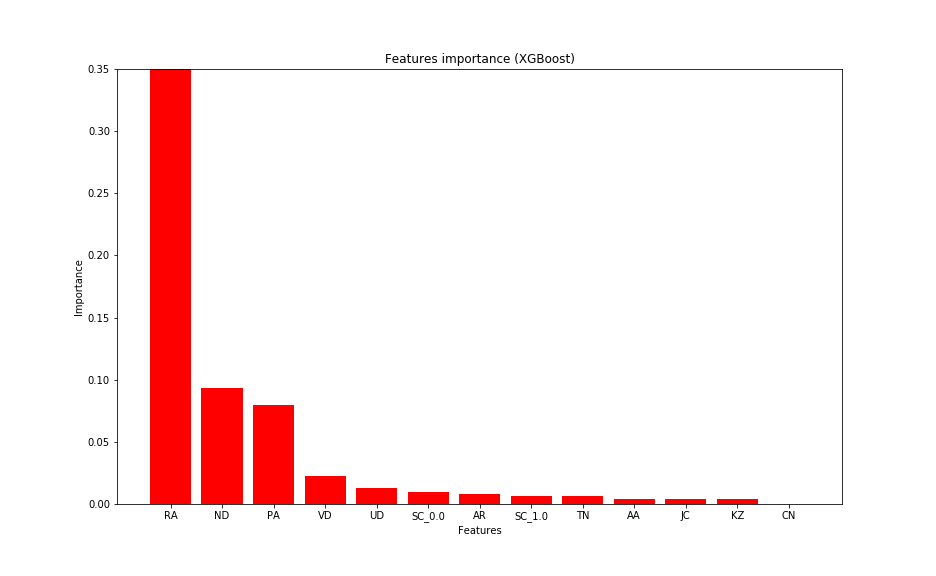
\includegraphics[width=15cm]{images/feature.png}
	\centering
	\caption{Features Importance.}\label{feature}
\end{figure}\\
As shown in figure\ref{feature}, Resource Allocation Index contributes most to the training with an importance of 0.35, which is two times larger than the second one. Followed by Neighborhood Distance and Preferential Attachment, they have almost the same contribution at around 0.10. The remaining methods are not so significant as their importance scores are near 0, they may be removed from the feature list.    \\


\section{Results and Comparison}
In this project, we use five classical similarity algorithm and a machine learning method GBDT to do the link prediction and recommend new friends for users. In order to verify the accuracy of these algorithm, the data set $E$ is randomly divided into two parts: a) the training set $E^T$, which is used as known information for calculation and training; b) the test set $E^A$, which is used for testing, the information in this collection cannot be used to train. Obviously, $E = E^T \cup E^A$ and $E^T \cap E^A = \varnothing$. In this project, the training set and test set are divided into 8:2, and AUC indicator is used to measure the accuracy of these algorithm. If all results are randomly generated, AUC = 0.5. Therefore, the degree of AUC > 0.5 measures how much the algorithm is more accurate than the method of random selection. The table \ref{result_t} shows the AUC for the different methods we have used, and the figure \ref{result_t} shows the ROC curves of these methods.
\begin{table}[h]
	\centering
	\caption{AUC Score of Different Algorithms}
	\label{result_t}
	\begin{tabular}{cccccccc}

		\hline

		Algorithm & GBDT & CN & JC &  AA & PA & Katz & Random Score \\

		\hline

		AUC& 0.96 & 0.88 & 0.91  & 0.91 & 0.52 & 0.86 & 0.5 \\

		\hline

	\end{tabular}

	
\end{table}

\begin{figure}[h!]
	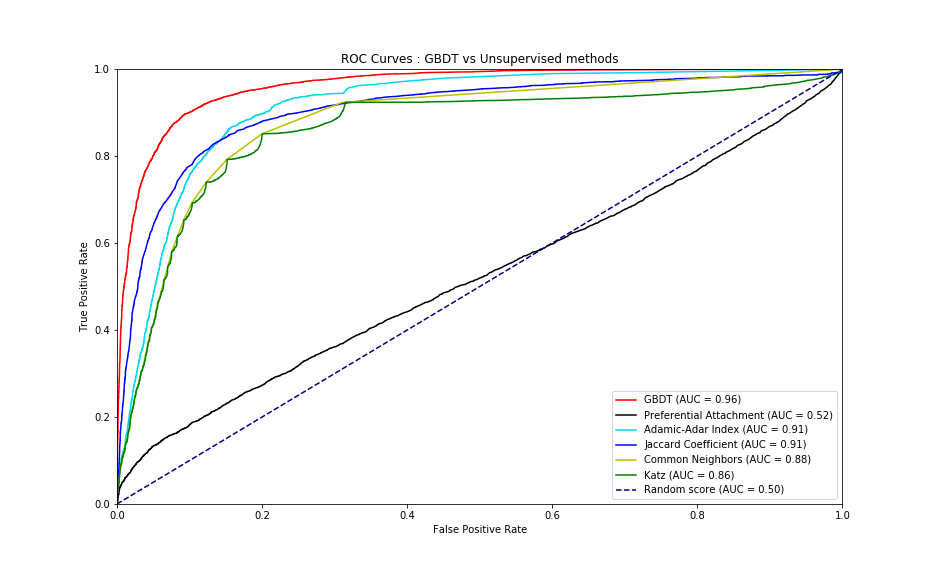
\includegraphics[width=13cm]{images/result.png}
	\centering
	\caption{ROC Curves of Different Algorithms.}	\label{result_fg}
\end{figure}

It can be seen from Table \ref{result_t} that the AUC score of GDBT (0.96) is the highest, and the accuracy is relatively high, followed by AA (Adamic/Adar index) and JC (Jaccard coefficient) whose AUC score (0.91) are also high. CN (Common neighbor) and katz (katz index) performed well with scores of 0.88 and 0.86 respectively. Among them, PA (Preferential Attachment) has the worst performance, only 0.52, and its accuracy is not much higher than random selection. From the ROC curves in Figure \ref{result_fg}, the accuracy of different algorithms is more obvious, and the performance of GBDT is the best.

\section{Conclusion}
In this project, we implemented a social network link prediction method based on GBDT, and implemented five traditional link prediction methods. The experimental comparison of these six methods on Facebook's dataset shows that the method based on GBDT is better than other traditional methods, and it can achieve better performance of link prediction.


\section*{References}


\small

[1] SARUKKAI R R. Link prediction and path analysis using markov chains[J]. Computer Networks, 2000, 33(1-6): 377-386.


[2]  ZHU J, HONG J, HUGHES J G. Using markov chains for link prediction in adaptive web sites[J]. Lect Notes Comput Sci, 2002, 2311:60-73.


[3]  POPESCUL A, UNGAR L. Statistical relational learning for link prediction[C]//Proceedings of the Workshop on Learning Statistical Models from Relational Data. New YorkACM Press, 2003: 81-87.


[4]  O’MADADHAIN J, HUTCHINS J, SMYTH P. Prediction and ranking algorithms for event-based network data[C]// Proceedings of the ACM SIGKDD 2005. New York: ACM Press, 2005: 23-30.


[5] LIN D. An information-theoretic definition of similarity[C]// Proceedings of the 15th Intl Conf Mach. Learn.. San Francisco, Morgan Kaufman Publishers, 1998: 296-304.


[6] CLAUSET A, MOORE C, NEWMAN M E J. Hierarchical structure and the prediction of missing links in networks[J]. Nature, 2008, 453: 98-101. 


[7]  Lin Yao, Luning Wang, Lv Pan\ \& Kai Yao \ (206) Link Prediction Based on Common-Neighbors for Dynamic Social Network. {\it Procedia Computer Science 83}, pp.\ 82--89.

[8] JACCARD P. Étude comparative de la distribution florale dans uneportion des Alpes et des Jura[J]. Bulletin del la Société Vaudoise des Sciences Naturelles, 1901, 37: 547-579.
\end{document}
